\documentclass[11pt, a4paper]{article}

\usepackage{graphicx}
\usepackage[english]{babel}
\usepackage[utf8x]{inputenc}
\usepackage{amsmath}
\usepackage[a4paper,top=3cm,bottom=2cm,left=2cm,right=2cm,marginparwidth=1.75cm]{geometry}
\usepackage{amssymb}

\graphicspath{ {./images} }
\newcommand*{\qed}{\hfill\ensuremath{\quad\square}}%
\newcommand*{\rad}{\ensuremath{\,\text{rad}}}
\newcommand*{\R}{\ensuremath{\mathbb{R}}}

\makeatletter
\renewcommand*\env@matrix[1][*\c@MaxMatrixCols c]{%
  \hskip -\arraycolsep
  \let\@ifnextchar\new@ifnextchar
  \array{#1}}
\makeatother

\newtheorem{theorem}{Theorem}

%------------------------------------------------
%Templates for images and figures
% \begin{figure}[h]
%   \centering
%   \subfloat[caption 1]{{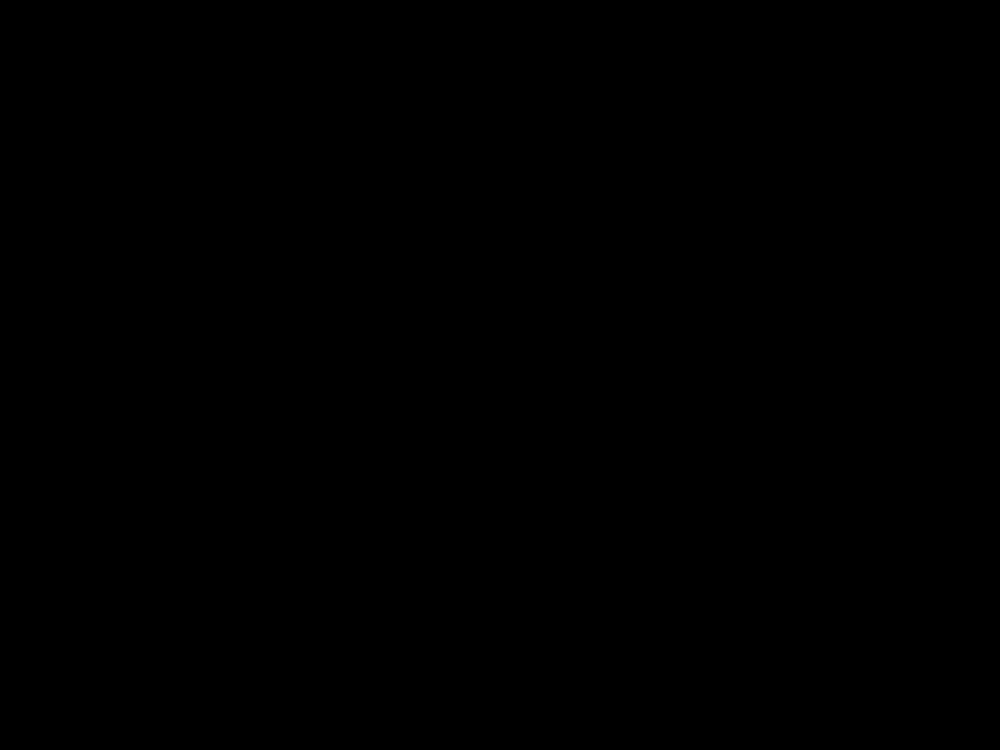
\includegraphics[width=30mm]{images/placeholder.png}}}%
%   \qquad
%   \subfloat[caption 2]{{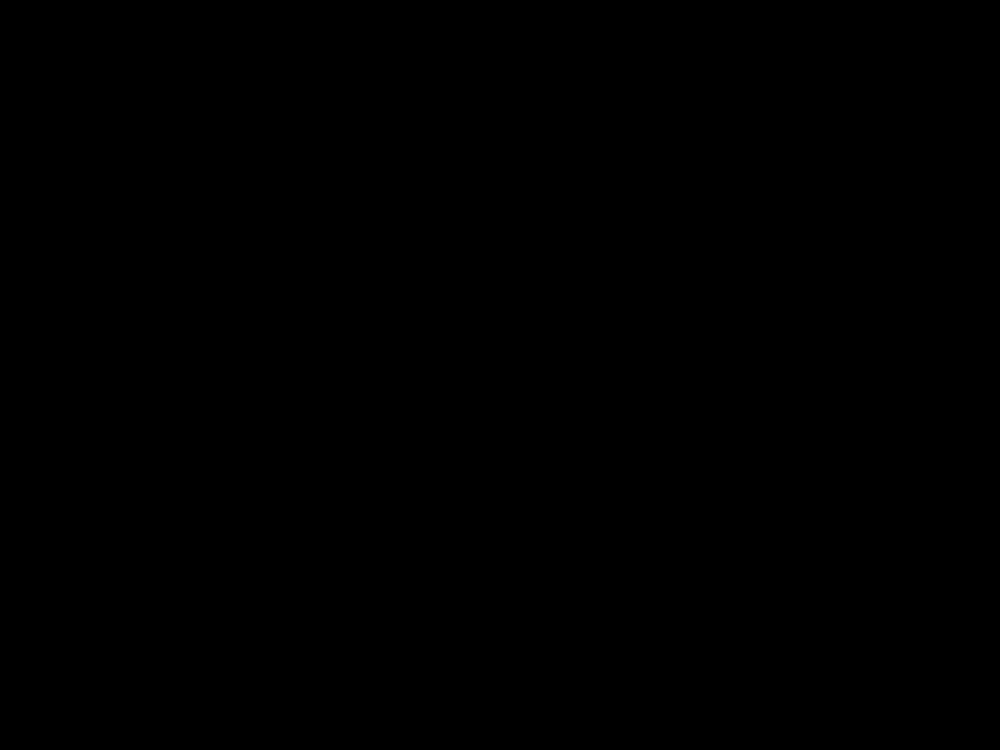
\includegraphics[width=30mm]{images/placeholder.png}}}%
%   \caption{Description}
% \end{figure}

% \begin{figure}[h]
%   \centerline{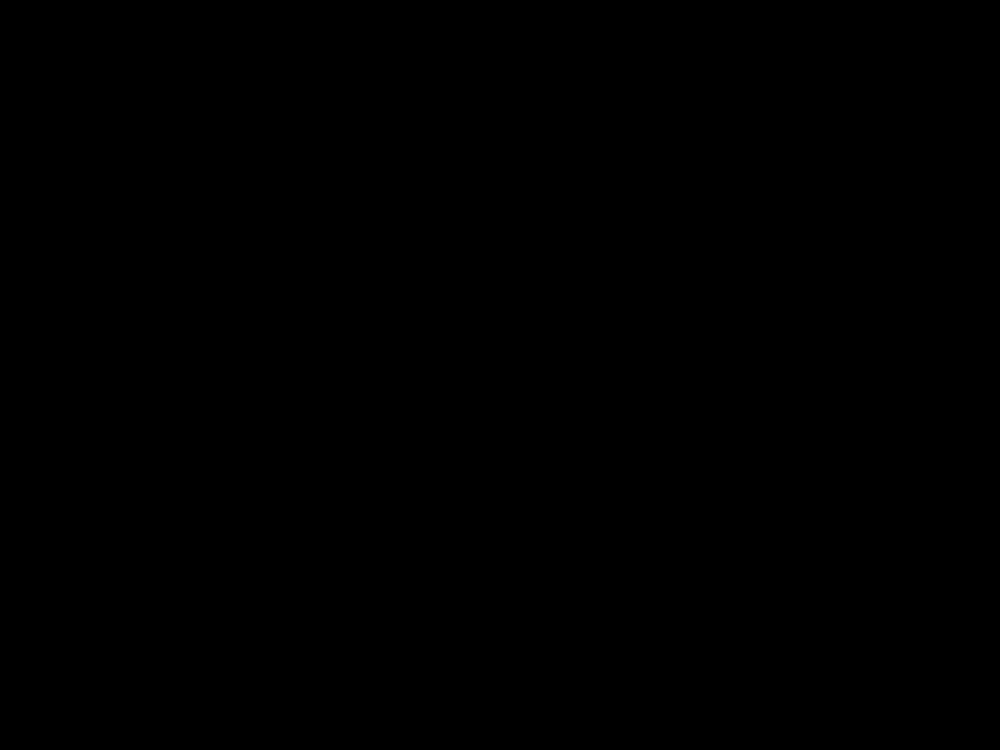
\includegraphics[width=50mm]{images/placeholder.png}}
%   \caption{Description}
% \end{figure}
%-----------------------------------------------

\begin{document}

\setcounter{section}{13}
\section{Energy methods for rigid bodies}
\subsection{Extension to rotations}
This lecture doesnt cover any real new material in all honesty. Energy methods for rigid bodies are identical to energy methods  or particles and point masses with the only difference being that now rotations are also considered. Thus:
\begin{equation}
  T_1 + V_1 + \Sigma U = T_2 + V_2
\end{equation}
Where $T=$Kinetic energy and $V=$potential energy. The new terms for potential and kinetic energy when considering translations and rotations will be as follows:
\begin{gather}
  T = \frac{1}{2}mv^2 + \frac{1}{2}I_G\omega^2\\
  V = mgh + \frac{1}{2}ks^2 + \frac{1}{2}k_r\theta^2\\
  U = \int_{s_1}^{s_2} F\,ds + \int_{\theta_1}^{\theta_2} M\,d\theta
\end{gather}
Equation (1) in it's most general form then becomes:
\begin{equation}
  \frac{1}{2}mv_1^2 + \frac{1}{2}I_G\omega_1^2 + mgh_1 + \frac{1}{2}ks_1^2 + \frac{1}{2}k_r\theta_1^2 +\int_{s_1}^{s_2} F\,ds + \int_{\theta_1}^{\theta_2} M\,d\theta =  \frac{1}{2}mv_2^2 + \frac{1}{2}I_G\omega_2^2 + mgh_2 + \frac{1}{2}ks_2^2 + \frac{1}{2}k_r\theta_2^2
\end{equation}


\end{document}